\subsection{Verfahren}
\label{superpixel_verfahren}

In der Literatur finden sich zahlreiche Verfahren zur Bestimmung einer Superpixelrepräsentation aus einem Bild mit jeweils unterschiedlichen Stärken und Schwächen~\cite{super, slic}.
Zwei beliebte Verfahren, die aufgrund ihrer im Allgemeinen guten Resultate bei geringer Berechnungskomplexität immer wieder zu finden sind, sind der SLIC- sowie der Quickshift-Algorithmus~\cite{slic, super, Gadde, supercnn, Fulkerson}.
Beide Verfahren werden im Folgenden näher vorgestellt.

\paragraph{SLIC}
\label{slic}

Der Superpixelalgorithmus \emph{\gls{SLIC}} ist ein recht einfach gehaltener lokaler \emph{$K$-Means}-Clustering-Ansatz, welcher sich dennoch durch seine Geschwindigkeit, seine Speichereffizienz und insbesondere durch seine erfolgreiche Segmentierung hinsichtlich der Farbabgrenzen seiner Superpixel im Vergleich zu anderen \enquote{State-of-the-Art}-Algorithmen auszeichnet~\cite{slic, Gadde}.

Ein Bild $\gls{B} \in \gls{R}^{H \times C \times 3}$ im \emph{Lab-Farbraum} wird dazu initial in $K \in \gls{N}$ viele Clusterzentren $\ve{c}_k \coloneqq {\left[l_k, a_k, b_k, x_k, y_k\right]}^{\top}$  mit jeweils gleichmäßigem Abstand $S \coloneqq \sqrt{WH/K}$ zerlegt~\cite{slic}.
Daraufhin werden in einem iterativen Prozess die Zugehörigkeiten der Pixel zu ihren jeweiligen Clustern über eine Distanzmetrik $D$ bestimmt und die Clusterzentren entsprechend ihrer neuen Gruppierungen angepasst.
Entgegen der konventionellen $k$-Means-Formulierung werden dabei aber nicht die Distanzen jedes Pixels zu jedem Clusterzentrum berechnet, sondern lediglich für die Pixel, die sich in der Region der Größe $2S \times 2S$ um $\ve{c}_k$ befinden~\cite{slic}.
Dies führt folglich zu einer drastischen Reduzierung der Anzahl an Distanzberechnungen und zu einem effizienteren Algorithmus.
Wurde zu jedem Pixel dessen ähnlichstes Clusterzentrum bestimmt, werden die Zentren über die Durchschnittsbildung all seiner zugehörigen Pixel neu justiert.
Nach einer festgelegten Anzahl an Iterationsschritten (üblicherweise $10$) bricht der Algorithmus schließlich ab~\cite{slic}.
Das gesamte Verfahren ist in Algorithmus~\ref{alg:slic} zusammengefasst.

\begin{algorithm}[t]
\centering
\begin{algorithmic}
  \REQUIRE{} Bild $\gls{B} \in \gls{R}^{H \times W \times 3}$ im Lab-Farbraum, Anzahl der Cluster $K$
  \ENSURE{} Segmentierungsmaske $\gls{Smaske} \in \gls{N}^{H \times W}$
  \STATE{} Initialisiere $K$ Clusterzentren ${\left\{\ve{c}_k\right\}}_{k=1}^K$ mit gleichmäßigem Abstand $S$.
  \STATE{} $\gls{Smaske}_{yx} \leftarrow -1$ für jedes Pixel $\gls{B}_{yx}$ an $\left(x,y\right)$.
  \STATE{} $\ma{D}_{yx} \leftarrow \infty$ für jedes Pixel $\gls{B}_{yx}$ an $\left(x,y\right)$.
  \REPEAT{}
    \FOR{$\ve{c}_k \in {\left\{\ve{c}_k\right\}}_{k=1}^K$}
      \FOR{Pixel $\gls{B}_{yx}$ an $\left(x,y\right)$ in $2S \times 2S$ Region um $\ve{c}_k$}
        \STATE{} Berechne Distanz $D$ zwischen $\ve{c}_k$ und $\gls{B}_{yx}$.
        \IF{$D < \ma{D}_{yx}$}
          \STATE{} $\ma{D}_{yx} \leftarrow D$
          \STATE{} $\gls{Smaske}_{yx} \leftarrow k$
        \ENDIF{}
      \ENDFOR{}
    \ENDFOR{}
    \STATE{} Justiere Clusterzentren ${\left\{\ve{c}_k\right\}}_{k=1}^K$.
  \UNTIL{Endbedingung}
\end{algorithmic}
\caption[\gls{SLIC}]{\gls{SLIC}-Algorithmus, der eine Segmentierungsmaske $\gls{Smaske} \in \gls{N}^{H \times W}$ in den Ausmaßen des Eingabebildes $\gls{B} \in \gls{R}^{H \times W \times 3}$ über ein lokales $K$-Means-Clustering bei $K$ gleichmäßig verteilten initialen Clusterzentren generiert.}
\label{alg:slic}
\end{algorithm}

Die Distanzmetrik $D$ basiert auf der euklidischen Norm ${\left\|\cdot\right\|}_2$ im fünfdimensionalen Raum ${\left[l,a,b,x,y\right]}^{\top}$ auf den Farben und den Positionen der Pixel \bzw{} der Clusterzentren.
Dabei ergeben sich jedoch Inkonsistenten für unterschiedliche Superpixelgrößen.
Bei großen Superpixeln führt dies zu einer stärkeren Gewichtung der räumlichen Positionen der Superpixel, wohingegen bei kleinen Superpixeln genau das Gegenteil der Fall ist~\cite{slic}.
Es ist daher notwendig, die Distanzen der Positionen $D_S$ und Farben $D_F$ getrennt voneinander zu betrachten und mittels dem Abstand $S$ der initialen Clusterzentren und einer Normalisierungskonstante $F \in \gls{R}$ \bzgl{} der Gewichtung der Farben zu normieren.
Damit ergibt sich $D$ als~\cite{slic}
\begin{equation*}
\begin{split}
  D & \coloneqq \sqrt{{\left(\frac{D_S}{S}\right)}^2 + {\left(\frac{D_F}{F}\right)}^2}\\
  D_S & \coloneqq {\left\|{\left[x, y\right]}^{\top} - {\left[x_k, y_k\right]}^{\top}\right\|}_2\\
  D_F & \coloneqq {\left\|{\left[l, a, b\right]}^{\top} - {\left[l_k, a_k, b_k\right]}^{\top}\right\|}_2.
\end{split}
\end{equation*}
Die Normalisierungskonstante $F$ kann damit auch als Gewichtung zwischen der Form und den Farbabgrenzungen der Superpixel verstanden werden.
Falls $F$ sehr klein gewählt wird, respektieren die Superpixel Farbabgrenzungen besser, aber besitzen im Allgemeinen auch eine eher unreguläre Form~\cite{slic}.

Damit ist \gls{SLIC} ein $\gls{O}\left(WH\right)$ effizienter Algorithmus mit nur zwei frei wählbaren Parametern $K$ und $F$~\cite{slic}.
Viele Anwendungen im Bereich der Bildverarbeitung machen sich daher \gls{SLIC} zu Nutze (\vgl{}~\cite{Gadde, supercnn, super}).
Abbildung~\ref{fig:slic_quickshift} (a) zeigt ein Beispielresultat des \gls{SLIC}-Algorithmus bei unterschiedlich gewählten Anzahlen an Clusterzentren.

\begin{figure}[t]
\centering
\subfigure[\gls{SLIC}]{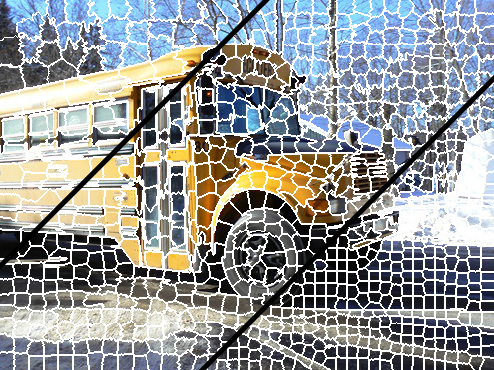
\includegraphics[scale=0.4]{bilder/slic_beispiel}}
\subfigure[Quickshift]{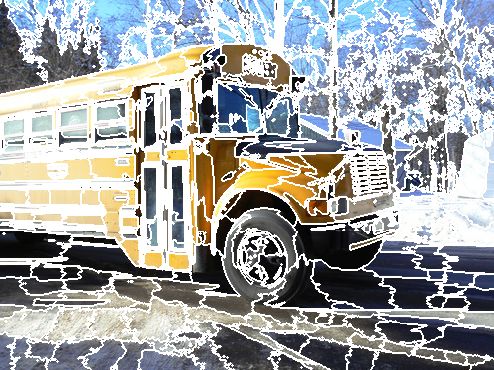
\includegraphics[scale=0.4]{bilder/quickshift_beispiel}}
  \caption[\gls{SLIC} und Quickshift Beispielresultat]{Ein Bus segmentiert über \gls{SLIC} mit jeweils 400, 800 und 1600 Superpixeln (a) sowie über Quickshift mit 600 Superpixeln (b).
  Dabei werden die unterschiedlichen Verfahren zur Generierung von Superpixeln deutlich.
  Wohingegen \gls{SLIC} möglichst quadratische, gleichgroße Superpixel erzeugt, wird die Form der Superpixel von Quickshift größtenteils über die Farbabgrenzungen gesteuert und erzeugt damit sowohl sehr große wie auch sehr kleine Superpixel in allen möglichen Variationen.}
\label{fig:slic_quickshift}
\end{figure}


\paragraph{Quickshift}
\label{quickshift}

Ein weiteres Verfahren zur Bildsegmentierung ist der gradientenbasierte Algorithmus \emph{Quickshift}, der unter anderem bereits zur Objektlokalisierung auf Basis von Superpixeln benutzt wurde~\cite{quickshift,Fulkerson}.

Quickshift startet dabei mit der Berechnung der \emph{Parzen-Dichteschätzung} $p$ eines Bildes $\gls{B} \in \gls{R}^{H \times W \times 3}$ für jedes Pixel $\gls{B}_{yx} \in \gls{R}^3$ im fünfdimensionalen Raum über die Gaußfunktion, \dhe{}
\begin{equation*}
  p\left(x,y, \gls{B}\right) = \sum_{\substack{1 \leq i \leq W\\1 \leq j \leq H}}
  \frac{1}{{\left(2\pi\gls{sigma}\right)}^5} \exp\left(-\frac{1}{2\gls{sigma}^2}{\left\|\begin{pmatrix}
    x - x_i\\
    y - y_i\\
    \alpha \left(\gls{B}_{yx} - \gls{B}_{y_i x_i}\right)
  \end{pmatrix}\right\|}_2^2\right),
\end{equation*}
mit der Standardabweichung $\gls{sigma} \in \gls{R}$ und der Gewichtung des Farbeinflusses über $\alpha \in \gls{R}$~\cite{quickshift}.
Je größer \gls{sigma} gewählt wird, umso größer wird der Anteil weitentfernter Pixel zu der Dichte des jeweils betrachteten Pixels.
In der Praxis kann, analog wie bei \gls{SLIC}, eine Fenstergröße $S \times S$ zur Einschränkung der Betrachtung der Pixel um einen Pixel definiert werden~\cite{super}.
Obwohl Quickshift standardmäßig $S$ auf $\infty$ setzt, lohnt es sich aus Effizienzgründen eine Größe in Abhängigkeit zu \gls{sigma} zu wählen~\cite{quickshift}.

Basierend auf den Dichten des Bildes generiert Quickshift einen Baum, der jedem Pixel $\gls{B}_{y_i x_i}$ seinen nächsten Nachbarn $\gls{B}_{y_j x_j}$ zuordnet, welcher einen höheren Dichtewert besitzt, \dhe{}
\begin{equation*}
  p\left(x_j, y_j, \gls{B}\right) > p\left(x_i, y_i, \gls{B}\right).
\end{equation*}
Falls $\gls{B}_{y_i x_i}$ kein solches Pixel zugeordnet werden kann, wird es mit keinem Pixel verbunden.
Die verbundene Menge an Knoten repräsentiert dann schließlich einen Superpixel des Bildes.

Quickshift segmentiert damit ein Bild auf Basis von drei Parametern — $\gls{sigma}$ für die  Standardabweichung der Gaußfunktion, $\alpha$ zur Gewichtung des Farbterms sowie $S$ zur Einschränkung der Berechnung über ein Fenster der Größe $S \times S$.
Die Superpixel, die Quickshift produziert, besitzen aber im Gegensatz zu den Superpixeln in \gls{SLIC} keine Einschränkung in ihrer Anzahl, Form oder Größe.
Ein segmentiertes Bild mit feinen Strukturen besitzt dann wohlmöglich weitaus mehr Superpixel, als ein Bild mit großen gleichfarbigen Flächen, welches nur sehr wenige, großflächige Superpixel generiert.
Ebenso gibt es im Gegensatz zu \gls{SLIC} keinen Parameter, der die Form der Superpixel steuern kann, sodass Quickshift Superpixel aller erdenklichen Formen produzieren kann.
Abbildung~\ref{fig:slic_quickshift} (b) illustriert ein Resultat einer Quickshift-Segmentierung und insbesondere den Vergleich zu dem entsprechenden \gls{SLIC}-Äquivalent.

\paragraph{Weitere Verfahren}
\label{weitere_superpixel_verfahren}

In den letzten Jahren wurden desweiteren zahlreiche eigenvektorbasierte Verfahren zur Bildsegmentierung entwickelt~\cite{super, felzenszwalb}.
Obwohl diese vielversprechende Resultate aufweisen, sind sie jedoch entsprechend langsam um von praktischem Nutzen für die meisten Anwendungen zu sein~\cite{felzenszwalb}.
Andere Algorithmen wiederum zeigen sich als besonders berechnungseffizient, liefern aber dementsprechend unzufriedenstellende Ergebnisse~\cite{felzenszwalb}.
Namenshaft zu erwähnen sei noch die \emph{effiziente graphbasierte Bildsegmentierung} von \citeauthor{felzenszwalb}, die in der Regel unter dem Namen \emph{Felzenszwalb-Segmentierung} bekannt ist~\cite{felzenszwalb}.
Der Algorithmus von \citeauthor{felzenszwalb} zeichnet sich dabei durch seine geringe Berechnungskomplexität aus und versucht gleichzeitig, globale Eigenschaften des Bildes zu erhalten.
Dafür wird das Bild als regulärer Gittergraph initialisiert, bei dem die Kantengewichte eine Aussage über den Unterschied in Helligkeit und Farbe der benachbarten Pixel treffen.
Der Algorithmus versucht daraufhin, Knoten insofern zu verschmelzen, dass der Unterschied zwischen den Kantengewichtungen innerhalb einer Region möglichst gering bleibt und zwischen benachbarten Regionen möglichst groß wird (\vgl{}~\cite{felzenszwalb}).
Die Felzenszwalb-Segmentierung zeigte sich aber in Tests auf einer Reihe von Bildern weniger geeignet, da dessen Parameter für jedes Bild eine spezielle Anpassung benötigen und folglich eine statische Wahl dieser Parameter zu unbrauchbaren Ergebnissen führte.
